\begin{figure}
	\centering
	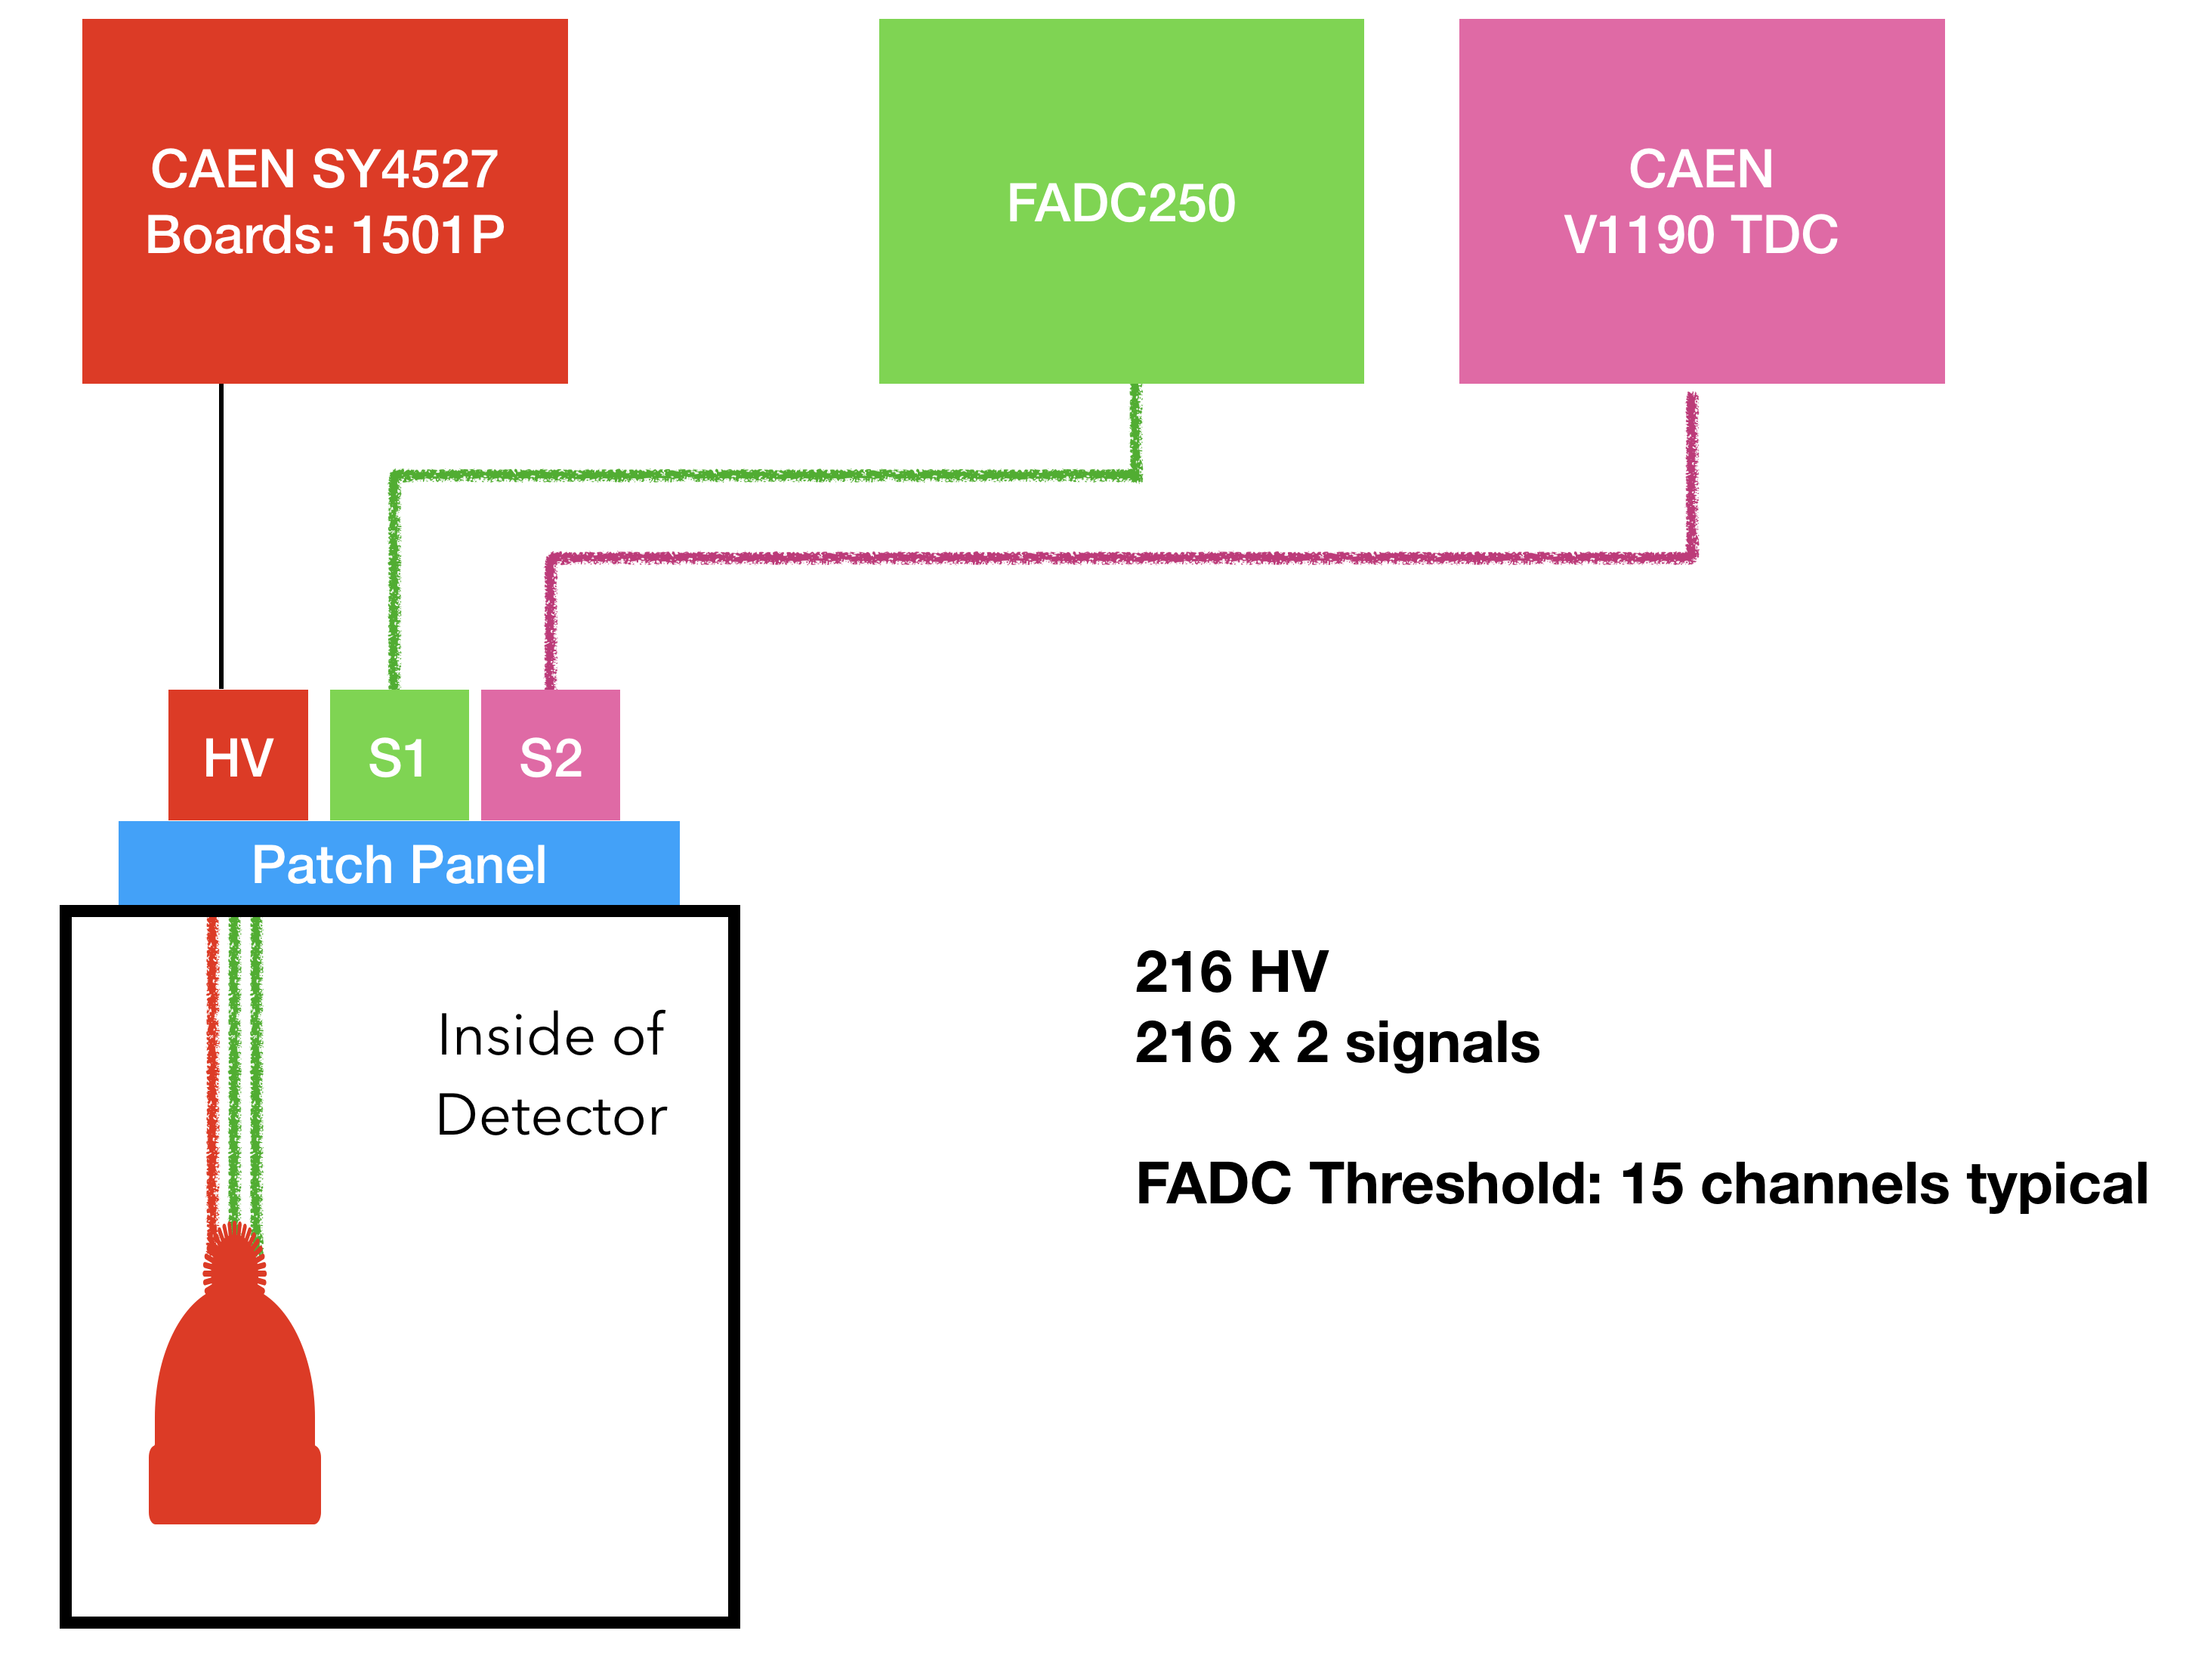
\includegraphics[width=0.99\columnwidth, height=0.6\columnwidth]{img/electronicScheme.png}
	\caption{The electronics schematic of the LTCC. One HV and two readout signals are connected from each PMT
          base to the patch panel. The patch panels then connect the HV to the CAEN SY4527 (1501P boards) and the
          PMT signals to the FADC250s and the DSC2 discriminators.}
	\label{fig:electronicScheme}
\end{figure}

\section{Electronics and Readout}

Figure~\ref{fig:electronicScheme} shows a schematic diagram of the electronics and readout used for the LTCC
detector. Since the magnetic shield case is near the bulb of the PMT, and the WC is in direct contact with the bulb,
the electrons in the PMT could strike the inner bulb wall if the negative voltage was applied to the cathode. For this
reason the signals are capacitatively coupled to positive HV, with the PMT cathode at ground potential. The
XP4500B Photonis PMTs anodes are powered with positive polarity by a CAEN SY4527 high voltage mainframe
outfitted with 1501P boards. There are two anode signals from the PMT output. One of them is connected directly to
flash ADC boards built at JLab, the Flash ADC module FADC250~\cite{daq-nim}. The FADC250 sampling
frequency is 250~MHz. The other signal is discriminated by the JLab-built discriminator scaler module DSC2
\cite{daq-nim}, and connected to CAEN v1190 TDC modules. The TDCs have a 50~ps/channel timing resolution, and
the discriminator threshold was set to 30~mV, corresponding to 15\% of the SPE amplitude. The LTCC FADC250 and
TDC information are read out using the CLAS12 Data Acquisition (DAQ) system~\cite{daq-nim}.

A typical signal from the FADC250 module is shown in \F{fadc}. The signal is usually contained in 3 to 5 time samples
(each time sample is 4~ns). In order to be written to tape, at least one of the 100 signal samples in the 400-ns wide
readout window must be above a threshold of 30 channels, corresponding to about 30\% of the SPE peak value.
This is well above the typical pedestal variation of 1-5 channels. The FADC250 then integrates the FADC signal over
a time window of 16~ns (4 samples) before the threshold crossing time, for the duration of 20 samples (80~ns). The
final integrated charge used in the reconstruction code is the signal integral minus the electronic pedestal, as
described in \F{fadc}.

\begin{figure}[H]
	\centering
	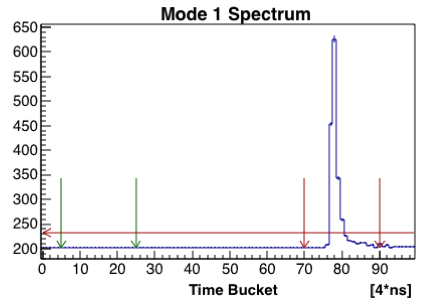
\includegraphics[width=0.99\columnwidth, height=0.6\columnwidth]{img/fadc.png}
	\caption{The FADC250 digitized output as a function of sample index for one of the LTCC PMTs.
          The DAQ system saves a 400~ns time window (100 samples) if at least one of the 100 signal samples is
          above a 30-channel threshold. The integral signal is the sum of the output at the sample indexes between
          the two right arrows, one placed 4 samples before the signal crosses the threshold, and the other placed
          20 samples after that. The final integrated charge used in the reconstruction code is this integral minus
          the pedestal. The pedestal is calculated using the average of the signal between the left arrows. The
          absolute positions of the pedestal acquisition limits and the relative position of the signal integration
          limits are adjusted in the DAQ parameters and loaded before each run.}
	\label{fig:fadc}
\end{figure}

